%%%%%%%%%%%%%%%%%%%%%%%%%%%%%%%%%%%%%%%%%%%%%%%%%%
\section{Statement of model}
The eukaryotic cell membrane acts as the main barrier between the cell and the surrounding environment. Inside the cell, the membrane is supported by a dense networks of actin filaments called the cortex which is attached to the cell membrane via adhesion molecules. The cortex maintains the cell shape and contracts inward generating a internal pressure in the cell. Local disruptions to the cortex result in dynamic, transient protrusions of the cell membrane termed blebs. Blebs are implicated in many cellular activities including apoptosis, mitosis and motility, yet little is known about the mechanism underlying bleb formation.
%%%%%%%%%%%%%%%%%%%%%%%%%%%%%%%%%%%%%%%%%%%%%%%%%%

\begin{figure}
   \begin{center}
   %\captionsetup{width=linewidth}
	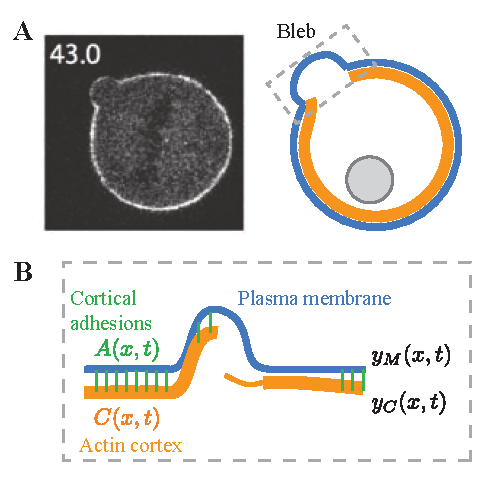
\includegraphics[width=8.5cm]{figs/figSchematic.pdf}
      \caption{(A) Micrograph of a single bleb, induced by laser ablation on the surface of a HeLa cell, 43 seconds after initial formation. Taken from \cite{Biro:2013bk}. (B) Model components. At each location on the surface of the cell $x$, four quantities are represented: The height of the membrane $y_M(x,t)$, the height and thickness of the actin cortex $y_C(x,t)$ and $C(x,t)$ respectively, and the local density of membrane-cortex anchoring proteins, $A(x,t)$. Note that the schematic shows the range of possible model states (e.g., thick or thin cortex, protruding or proximal membrane), while specific predicted dynamics will be determined by simulation.}
      \label{fig::schematic}
   \end{center}
\end{figure}

%%%%%%%%%%%%%%%%%%%%%%%%%%%%%%%%


Our minimal model, summarized schematically in Fig.~\ref{fig::schematic}, consists of four fundamental dynamic variables, as functions of time $t$ and location on the two-dimensional cell surface, parametrized by $(x_1, x_2)$. The actin cortex, has local height described by $Y_C(x_1,x_2,t)$ measured normal to the mean cell surface from its steady-state configuration $Y_C=0$, and thickness $C(x_1,x_2,t)$. The cortical-cytoplasmic actin cytoskeleton can in principle have complicated morphologies that cannot be accounted for by a single location $Y_C$, so we think of $Y_C$ as the weighted average position of maximal cortical actin. Membrane-cortex adhesions are described by density $A(x_1,x_2,t)$ in molecules/ $\text{nm}^2$. Finally, the plasma membrane has local height $Y_M(x_1,x_2,t)$.
%%%%%%%%%%%%%%%%%%%%%%%%%%%%%%%%%%%%%%%%%%%%%%%%%%
%\subsection{Derivation, reduction to one dimensions, and non-dimensionalization}

\subsection{Derivation, and non-dimensionalization}
The dynamics of the actin cortex and  density of adhesions attaching cortex and membrane are governed by
\begin{align}
\dot{C} &= \omega A - \gamma C \label{eq::CDotequation}\\
\dot{A} &=  \frac{\kon\,C}{C_0+C}\; \mbox{exp}\left( - \left(\frac{y-Y_C}{\delta}\right)\right) - \koff A\; \mbox{exp}\left( \frac{k_A (Y_M-Y_C)}{F}\right)\label{eq::ADotequation}
\end{align}

Balance of forces on the cortex is determined by adhesions, which pull the cortex outwards (towards the membrane), and myosin, which contracts, pulling the cortex inwards (towards the cell body):
\begin{align}
0 &= A k_A (Y_M-Y_C) - \sigma_M C Y_C \label{eq::forceBalanceCortex}
\end{align}
Balance of forces on membrane is determined by adhesions, which pull the cortex inwards, and hydrostatic pressure, which pushes the membrane out. 
\begin{align}
0 &= - Ak_A (Y_M-Y_C) + \hat{\Pi}(Y_M^0 - Y_M) + \gamma_M \nabla^2  Y_M \label{eq::forceBalanceMembrane}
\end{align}
Since mechanical equilibration is fast, $Y_M(t)$ and $Y_C(t)$ always evolve to satisfy these equations.


The resulting dimensionless system is:
\begin{align}
\dfrac{dc}{dt}  & =  \Omega a - c\label{eq::nondimc}\\
\epsilon\dfrac{da}{ dt}  & =  \dfrac{c}{1+c} \mbox{exp}\left(-\dfrac{y-y_C}{D}\right) - a \mbox{exp} \left(\dfrac{y-y_C}{F} \right)\label{eq::nondima}\\
0 & = a(y-y_C) - Mcy_C\label{eq::nondimyC}\\
0 & = -a(y - y_C) + P (1-y) + \dfrac{\partial^2 y}{\partial x^2}\label{eq::nondimyM}
\end{align}

%%%%%%%%%%%%%%%%%%%%%%%%%%%%%%%%%%%%%%%%%%%%%%%%%%
\subsection{Formulation as non-local integro-PDE}
%%%%%%%%%%%%%%%%%%%%%%%%%%%%%%%%%%%%%%%%%%%%%%%%%%
Equations ~\ref{eq::nondimc} - ~\ref{eq::nondimyM} can be represented as an integro-PDE. Eq. ~\ref{eq::nondimyM} is a self adjoint. It is very difficult or impossible to find a closed form solution. If we assume a solution exists and has the form $y(x,t) = \int_x h(s,t) ds + r(x,t)$, the we can rewrite the system as:



%%%%%%%%%%%%%%%%%%%%%%%%%%%%%%%%%%%%%%%%%%%%%%%%%%
\subsection{Connections to a larger class of models arising in cell mechanics}
%%%%%%%%%%%%%%%%%%%%%%%%%%%%%%%%%%%%%%%%%%%%%%%%%%